\chapter{Polimer}\label{ch:g12:polymers}

Jaket bulu sintetis dapat dipintal dari botol-botol minuman yang
dilelehkan; tali panjat tebing dibuat dari nilon; halaman ini adalah
selulosa, yang dibuat oleh pohon. Ketiganya adalah \omterm{def:g12:polymers:polymer}{polimer}:
\omterm{def:g7:atoms-and-molecules:molecule}{molekul-molekul} sepanjang ribuan \omterm{def:g7:atoms-and-molecules:atom}{atom}, yang dibangun dengan mengulang
satu satuan kecil berkali-kali. Sifat-sifatnya --- lunak atau kaku,
lentur atau rapuh, dapat dilelehkan atau tidak --- tidak terlalu
ditentukan oleh \omterm{def:g7:atoms-and-molecules:atom}{atom-atom} yang dikandungnya, melainkan oleh cara rantai
panjangnya tersusun.

\begin{recall}
\omterm{def:g8:plastics:plastic}{Plastik} tersusun atas \omterm{def:g7:atoms-and-molecules:molecule}{molekul-molekul} yang sangat panjang; \omterm{def:g8:plastics:thermoplastic}{termoplastik}
melunak jika dipanaskan, \omterm{def:g8:plastics:thermoplastic}{termoset} tidak (\cref{ch:g8:plastics}). Gugus
\omterm{def:g11:functional-groups:alcohol}{alkohol}, asam, \omterm{def:g11:functional-groups:carboxylic-acid}{ester}, \omterm{def:g11:functional-groups:amine}{amina}, dan \omterm{def:g11:functional-groups:amine}{amida}
(\cref{ch:g11:functional-groups}). \omterm{def:g12:curly-arrows:categories}{Adisi} menggabungkan dua \omterm{def:g7:atoms-and-molecules:molecule}{molekul}
menjadi satu tanpa kehilangan satu \omterm{def:g7:atoms-and-molecules:atom}{atom} pun
(\cref{ch:g12:curly-arrows}).
\end{recall}

\begin{omfigure}
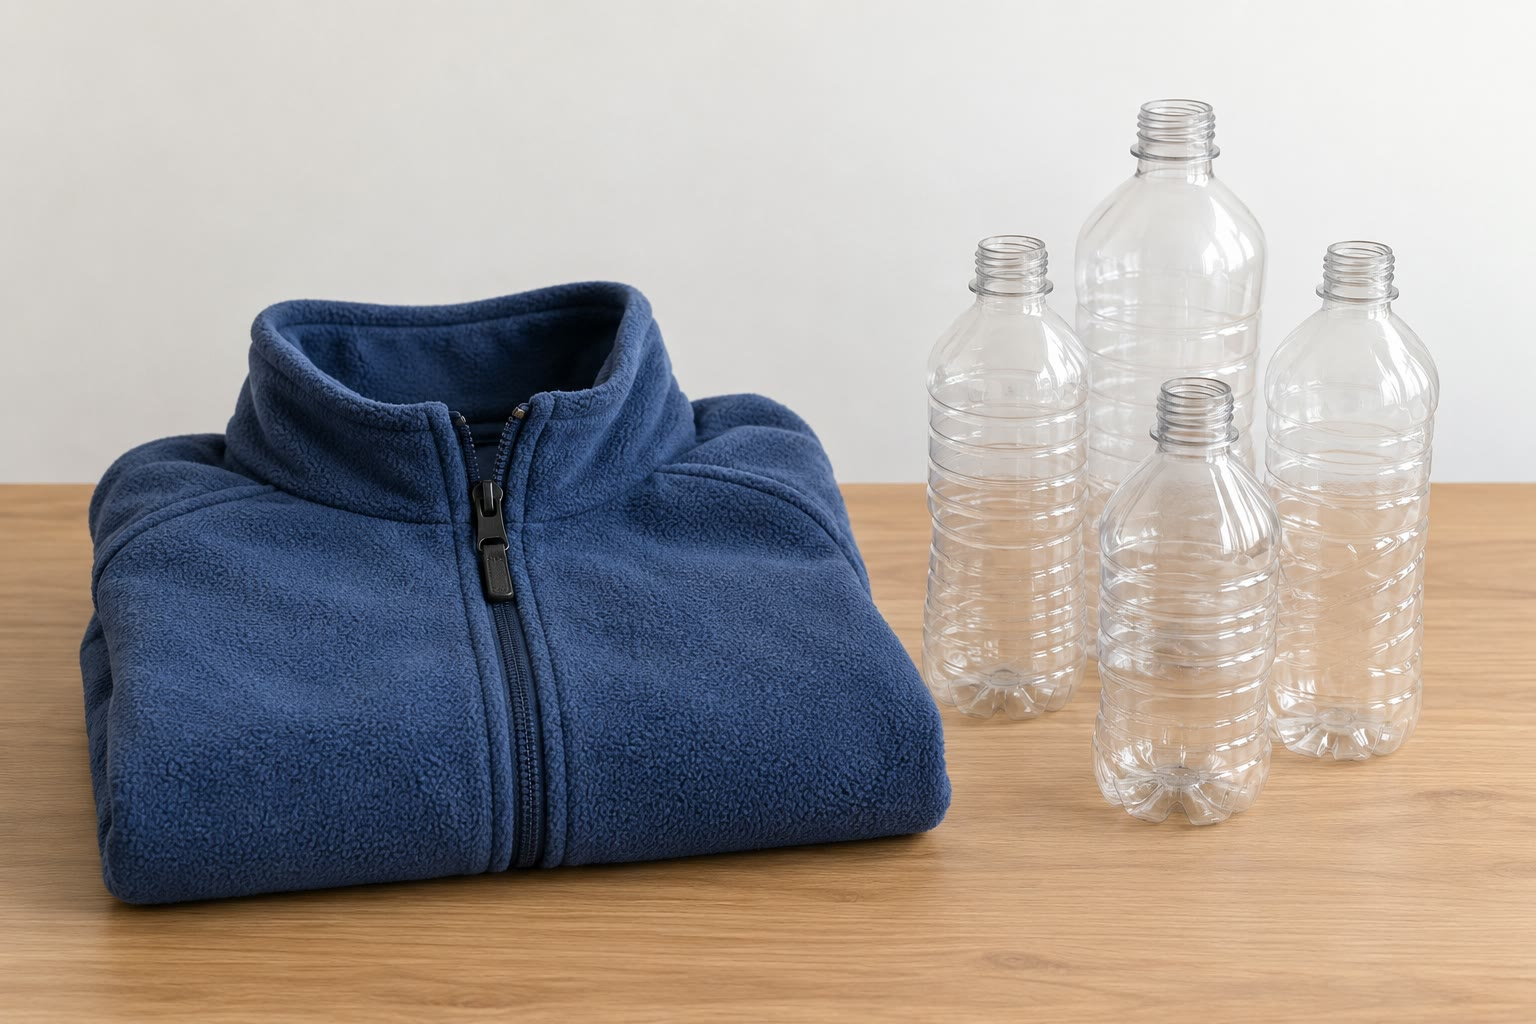
\includegraphics[width=0.45\linewidth]{images/book1/ai/g12-fleece-bottles.jpg}

{\small Botol minuman bekas dan jaket bulu sintetis: \omterm{def:g12:polymers:polymer}{polimer} yang sama,
dalam dua bentuk.}
\end{omfigure}

\section{Monomer, polimer, unit ulang}

\begin{definition}[Polimer, monomer, polimerisasi]\label{def:g12:polymers:polymer}
Yang disebut \emph{polimer}\index{polimer} adalah zat yang tersusun atas
\omterm{def:g7:atoms-and-molecules:molecule}{molekul-molekul} yang sangat besar, yaitu makromolekul, yang
masing-masing dibangun dari banyak satuan kecil yang terikat satu demi
satu. \omterm{def:g7:atoms-and-molecules:molecule}{Molekul-molekul} kecil pembentuknya disebut
\emph{monomer}\index{monomer}-nya; reaksi yang menggabungkannya disebut
\emph{polimerisasi}\index{polimerisasi}.
\end{definition}

\begin{definition}[Unit ulang, derajat polimerisasi]\label{def:g12:polymers:repeat-unit}
Yang disebut \emph{unit ulang}\index{unit ulang} sebuah \omterm{def:g12:polymers:polymer}{polimer} adalah
kelompok \omterm{def:g7:atoms-and-molecules:atom}{atom} terkecil yang pengulangannya menghasilkan rantai itu; unit
ini ditulis di antara kurung dengan indeks $n$. Banyaknya unit ulang $n$
dalam sebuah rantai disebut
\emph{derajat polimerisasi}\index{derajat polimerisasi}-nya.
\end{definition}

\begin{omfigure}
\[
  n\;\ce{CH2=CH2}
  \quad\longrightarrow\quad
  \chemfig{-[@{op1,.75}]CH_2-CH_2-[@{cl1,0.25}]}
  \polymerdelim[height=6pt, depth=6pt, indice=n]{op1}{cl1}
\]

{\small \omterm{def:g12:polymers:polymer}{Polimerisasi} etena: $n$ \omterm{def:g7:atoms-and-molecules:molecule}{molekul} \omterm{def:g12:polymers:polymer}{monomer} menghasilkan satu rantai
polietena, yang \omterm{def:g12:polymers:repeat-unit}{unit ulangnya} \ce{-CH2-CH2-} ditulis di antara kurung.}
\end{omfigure}

\begin{proposition}[Massa molar polimer]\label{prop:g12:polymers:molar-mass}
Rantai dengan \omterm{def:g12:polymers:repeat-unit}{derajat polimerisasi} $n$ memiliki \omterm{def:g10:the-mole:molar-mass}{massa molar}
\[
  M(\text{polimer}) \approx n \times M(\text{unit ulang}) ,
\]
karena kedua ujung rantai dapat diabaikan untuk $n$ yang besar.
\end{proposition}

\begin{proof}
Rantai itu terdiri atas $n$ \omterm{def:g12:polymers:repeat-unit}{unit ulang} ditambah dua gugus ujung yang
masing-masing beberapa \omterm{def:g7:atoms-and-molecules:atom}{atom}; untuk $n$ dalam orde ribuan, gugus-gugus
ujung itu beratnya kurang dari seperseribu keseluruhannya.
\end{proof}

\begin{example}[Sebuah rantai polietena]\label{ex:g12:polymers:pe}
% ledger: aw:C, aw:H
Rantai polietena dengan \omterm{def:g10:the-mole:molar-mass}{massa molar} \qty{280000}{g/mol} memiliki
$n = 280000/28.0 = 10000$ \omterm{def:g12:polymers:repeat-unit}{unit ulang}, jadi dua puluh ribu \omterm{def:g7:atoms-and-molecules:atom}{atom} karbon
berderet. Dalam sampel nyata, rantai-rantainya tidak semuanya sama
panjang: $n$ adalah nilai rata-rata.
\end{example}

\section{Polimer adisi}

\begin{definition}[Polimer adisi, polimer kondensasi]\label{def:g12:polymers:addition-polymer}
Sebuah \emph{polimer adisi}\index{polimer adisi} terbentuk melalui \omterm{def:g12:curly-arrows:categories}{adisi}
\omterm{def:g12:polymers:polymer}{monomer-monomer} yang membawa \omterm{def:g10:lewis-and-shape:multiple-bond}{ikatan rangkap} \ce{C=C}, tanpa produk lain:
\omterm{def:g12:polymers:repeat-unit}{unit ulangnya} memiliki \omterm{def:g7:atoms-and-molecules:atom}{atom-atom} yang sama dengan \omterm{def:g12:polymers:polymer}{monomernya}. Sebuah
\emph{polimer kondensasi}\index{polimer kondensasi} terbentuk melalui
reaksi antara dua \omterm{def:g11:functional-groups:functional-group}{gugus fungsi} yang menggabungkan dua \omterm{def:g12:polymers:polymer}{monomer} dan
melepaskan sebuah \omterm{def:g7:atoms-and-molecules:molecule}{molekul} kecil, biasanya air, pada setiap
sambungannya.
\end{definition}

\begin{omfigure}
\footnotesize
\renewcommand{\arraystretch}{1.5}
\begin{tabular}{l l l l}
\hline
\omterm{def:g12:polymers:polymer}{monomer} & \omterm{def:g12:polymers:polymer}{polimer} & \omterm{def:g12:polymers:repeat-unit}{unit ulang} & kegunaan \\
\hline
etena \ce{CH2=CH2} & polietena (PE) & \ce{-CH2-CH2-} & kantong, botol \\
kloroetena \ce{CH2=CHCl} & poli(vinil klorida) (PVC) & \ce{-CH2-CHCl-} & pipa, kusen \\
feniletena \ce{CH2=CH-C6H5} & polistirena (PS) & \ce{-CH2-CH(C6H5)-} & gelas, busa \\
tetrafluoroetena \ce{CF2=CF2} & PTFE & \ce{-CF2-CF2-} & panci antilengket \\
\hline
\end{tabular}\par\medskip

{\small Empat \omterm{def:g12:polymers:addition-polymer}{polimer adisi}. Pada masing-masing, \omterm{def:g10:lewis-and-shape:multiple-bond}{ikatan rangkap} \omterm{def:g12:polymers:polymer}{monomer}
terbuka, dan kedua karbonnya bergabung ke dalam rantai.}
\end{omfigure}

\begin{method}[Menemukan monomer dari sebuah polimer]\label{met:g12:polymers:monomer}
\begin{enumerate}
  \item Temukan \omterm{def:g12:polymers:repeat-unit}{unit ulangnya}: kelompok terkecil yang pengulangannya
        menghasilkan rantai itu.
  \item Jika rantai utamanya hanya berisi \omterm{def:g7:atoms-and-molecules:atom}{atom} karbon, \omterm{def:g12:polymers:polymer}{polimer} itu
        \omterm{def:g12:polymers:addition-polymer}{polimer adisi}: kembalikan \omterm{def:g10:lewis-and-shape:multiple-bond}{ikatan rangkap} di antara kedua karbon
        rantai utama \omterm{def:g12:polymers:repeat-unit}{unit ulangnya}. Itulah \omterm{def:g12:polymers:polymer}{monomernya}.
  \item Jika rantai utamanya berisi sambungan \omterm{def:g11:functional-groups:carboxylic-acid}{ester} atau \omterm{def:g11:functional-groups:amine}{amida}, \omterm{def:g12:polymers:polymer}{polimer}
        itu \omterm{def:g12:polymers:addition-polymer}{polimer kondensasi}: potonglah setiap sambungan, lalu
        kembalikan kepada setiap sisi \omterm{def:g7:atoms-and-molecules:atom}{atom-atom} \omterm{def:g7:atoms-and-molecules:molecule}{molekul} kecil yang
        dilepaskan (\ce{-OH} kepada \ce{C=O}, \ce{-H} kepada \ce{O} atau
        \ce{N}). Itulah \omterm{def:g12:polymers:polymer}{monomer-monomernya}.
\end{enumerate}
\end{method}

\begin{example}[Monomer PVC]\label{ex:g12:polymers:pvc}
Rantai \omterm{def:g12:polymers:polymer}{polimer} ini, \ce{-CH2-CHCl-CH2-CHCl-CH2-CHCl-}, mengulang
\ce{-CH2-CHCl-};
rantai utamanya hanya berisi karbon, jadi \omterm{def:g12:polymers:polymer}{monomernya} adalah
\ce{CH2=CHCl}, kloroetena.
\end{example}

\section{Polimer kondensasi}

\omterm{def:g12:polymers:polymer}{Monomer} dengan satu gugus reaktif hanya dapat berikatan sekali: \omterm{def:g12:polymers:polymer}{monomer}
itu mengakhiri rantai. Untuk membangun rantai melalui kondensasi, setiap
\omterm{def:g12:polymers:polymer}{monomer} memerlukan dua gugus, satu di setiap ujungnya.

\begin{example}[PET, sebuah poliester]\label{ex:g12:polymers:pet}
% ledger: aw:C, aw:H, aw:O
Etana-1,2-diol, \ce{HO-CH2-CH2-OH}, membawa dua gugus \omterm{def:g11:functional-groups:alcohol}{alkohol}; asam
benzena-1,4-dikarboksilat, \ce{HOOC-C6H4-COOH}, membawa dua gugus asam.
Setiap gugus asam membentuk \omterm{def:g11:functional-groups:carboxylic-acid}{ester} dengan sebuah gugus \omterm{def:g11:functional-groups:alcohol}{alkohol} dan
melepaskan air: rantainya tumbuh dari kedua ujung. \omterm{def:g12:polymers:polymer}{Polimernya} adalah
poli(etilena tereftalat), PET, bahan botol minuman dan serat poliester.
\omterm{def:g12:polymers:repeat-unit}{Unit ulangnya}, \ce{C10H8O4}, memiliki \omterm{def:g10:the-mole:molar-mass}{massa molar} \qty{192.0}{g/mol},
yaitu massa kedua \omterm{def:g12:polymers:polymer}{monomer} ($62.0 + 166.0$) dikurangi dua \omterm{def:g7:atoms-and-molecules:molecule}{molekul} air
($36.0$).
\end{example}

\begin{omfigure}
\setchemfig{atom sep=1.9em}
\chemfig{HO-CH_2-CH_2-OH}
\quad $+$ \quad
\chemfig{HO-C(=[2]O)-*6(-=-(-C(=[2]O)-OH)=-=)}

\medskip
$\longrightarrow$\quad
\chemfig{-[@{op2,.75}]O-CH_2-CH_2-O-C(=[2]O)-*6(-=-(-C(=[2]O)-[@{cl2,0.25}])=-=)}
\polymerdelim[height=20pt, depth=6pt, indice=n]{op2}{cl2}
\quad $+\ 2n\ \ce{H2O}$

{\small PET dari kedua \omterm{def:g12:polymers:polymer}{monomernya}: setiap sambungan \omterm{def:g11:functional-groups:carboxylic-acid}{ester} (gugus
\ce{-CO-O-}) melepaskan satu \omterm{def:g7:atoms-and-molecules:molecule}{molekul} air.}
\end{omfigure}

\begin{example}[Nilon-6,6, sebuah poliamida]\label{ex:g12:polymers:nylon}
Heksana-1,6-diamina, \ce{H2N-(CH2)6-NH2}, dan asam heksanadioat,
\ce{HOOC-(CH2)4-COOH}, bergabung melalui sambungan \omterm{def:g11:functional-groups:amine}{amida}, yang
masing-masing melepaskan satu \omterm{def:g7:atoms-and-molecules:molecule}{molekul} air:
\[
  \cdots\ce{-NH-(CH2)6-NH-CO-(CH2)4-CO-}\cdots
\]
Kedua angka enam pada namanya menyatakan jumlah \omterm{def:g7:atoms-and-molecules:atom}{atom} karbon setiap
\omterm{def:g12:polymers:polymer}{monomer}. Sambungan-sambungan \omterm{def:g11:functional-groups:amine}{amida} rantai yang bersebelahan saling
menarik melalui \omterm{def:g11:polarity-and-cohesion:hydrogen-bond}{ikatan hidrogen}, yang membuat serat nilon kuat.
\end{example}

\begin{history}[Carothers dan nilon]
% ledger: hist:polyamides-1934, hist:nylon-production-1939
Ahli kimia Wallace Carothers, yang memimpin laboratorium penelitian
sebuah perusahaan kimia, bertekad membuktikan bahwa \omterm{def:g12:polymers:polymer}{polimer}
benar-benar \omterm{def:g7:atoms-and-molecules:molecule}{molekul} raksasa dan membuatnya secara sengaja. Timnya
mula-mula membuat poliester, yang terlalu mudah meleleh untuk berguna;
pada tahun 1934 mereka beralih ke \omterm{def:g11:functional-groups:amine}{amina} dan membuat poliamida, di
antaranya serat yang kemudian dinamai nilon. Nilon mulai diproduksi pada
tahun 1939, mula-mula sebagai stoking yang menggemparkan sebuah pameran
dunia, lalu sebagai parasut, tali, dan bulu sikat gigi.
\end{history}

\begin{omfigure}
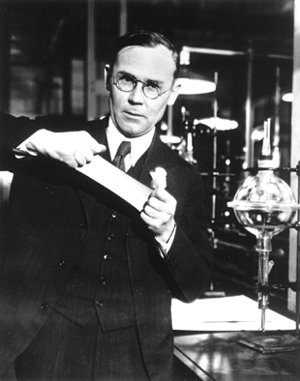
\includegraphics[width=0.24\linewidth]{images/book1/carothers.jpg}

{\small Wallace Carothers di laboratoriumnya.}
\end{omfigure}

\section{Struktur dan sifat}

Dua sampel dari \omterm{def:g12:polymers:polymer}{polimer} yang sama dapat berperilaku sangat berbeda: yang
menentukan adalah panjang rantainya, bentuknya, dan cara rantai-rantai
itu tersusun rapat.

\begin{proposition}[Rantai dan sifat]\label{prop:g12:polymers:properties}
\begin{itemize}
  \item Rantai yang lebih panjang lebih banyak terbelit: bahannya lebih
        kuat dan meleleh pada suhu yang lebih tinggi.
  \item Rantai linear dapat berjajar berdampingan dalam daerah yang
        teratur, \emph{kristalin}; rantai bercabang tidak dapat, dan
        tetap tidak teratur, \emph{amorf}. Daerah kristalin membuat
        \omterm{def:g12:polymers:polymer}{polimer} lebih rapat, lebih kaku, dan kurang bening.
  \item Rantai yang berdampingan hanya karena gaya antarmolekul saling
        bergeser jika dipanaskan: \omterm{def:g12:polymers:polymer}{polimernya} \omterm{def:g8:plastics:thermoplastic}{termoplastik}. Rantai yang
        dihubungkan oleh \emph{ikatan silang} kovalen tidak dapat
        bergeser: \omterm{def:g12:polymers:polymer}{polimernya} \omterm{def:g8:plastics:thermoplastic}{termoset}, atau, dengan sedikit ikatan
        silang, padatan elastis seperti karet.
\end{itemize}
\end{proposition}

\begin{proof}
Pemanasan memberi rantai-rantai itu cukup energi untuk mengatasi gaya
antarmolekul di antaranya (\cref{ch:g11:polarity-and-cohesion}), yang
lebih lemah daripada \omterm{def:g10:lewis-and-shape:covalent-bond}{ikatan kovalen}; makin banyak persentuhan
antarrantai, makin banyak energi yang diperlukan. Ikatan silang bersifat
kovalen: memutusnya merusak bahan itu alih-alih melelehkannya.
\end{proof}

\begin{omfigure}
\begin{tikzpicture}[font=\footnotesize, line width=1pt, line cap=round,
    lab/.style={below, align=center, text width=2.8cm}]
  % linear, packed (crystalline)
  \begin{scope}
    \foreach \y in {0,0.25,0.5,0.75,1.0}
      \draw[omDef] plot[smooth, domain=0:2.2, samples=25] (\x, {\y + 0.05*sin(400*\x)});
    \node[lab] at (1.1,-0.2) {rantai linear\\ berjajar: kristalin};
  \end{scope}
  % linear, tangled (amorphous)
  \begin{scope}[xshift=3.4cm]
    \draw[omDef] plot[smooth] coordinates {(0,0.2) (0.5,0.9) (1.0,0.3) (1.4,1.1) (2.0,0.5) (2.2,0.9)};
    \draw[omProp] plot[smooth] coordinates {(0,0.9) (0.4,0.3) (0.9,1.0) (1.5,0.2) (1.9,1.0) (2.2,0.3)};
    \draw[black!60] plot[smooth] coordinates {(0.1,0.55) (0.7,0.1) (1.2,0.75) (1.7,0.55) (2.2,0.1)};
    \node[lab] at (1.1,-0.2) {rantai linear\\ terbelit: amorf};
  \end{scope}
  % branched
  \begin{scope}[xshift=6.8cm]
    \draw[omDef] plot[smooth] coordinates {(0,0.5) (0.6,0.6) (1.2,0.45) (1.8,0.65) (2.2,0.5)};
    \draw[omDef] (0.5,0.6) -- (0.35,1.05) (1.0,0.5) -- (1.15,0.05) (1.6,0.6) -- (1.5,1.1) (1.6,0.6) -- (1.95,1.0);
    \node[lab] at (1.1,-0.2) {rantai bercabang:\\ tidak dapat rapat};
  \end{scope}
  % cross-linked
  \begin{scope}[xshift=10.2cm]
    \foreach \y in {0.1,0.55,1.0}
      \draw[omDef] plot[smooth, domain=0:2.2, samples=25] (\x, {\y + 0.06*sin(300*\x)});
    \foreach \x/\a/\b in {0.4/0.1/0.55, 1.3/0.1/0.55, 0.9/0.55/1.0, 1.9/0.55/1.0}
      \draw[omProp, line width=1.6pt] (\x,\a) -- (\x,\b);
    \node[lab] at (1.1,-0.2) {rantai berikatan silang:\\ tidak meleleh};
  \end{scope}
\end{tikzpicture}

{\small Empat susunan rantai \omterm{def:g12:polymers:polymer}{polimer}. Ikatan silang (jingga) adalah
\omterm{def:g10:lewis-and-shape:covalent-bond}{ikatan kovalen} antarrantai.}
\end{omfigure}

\begin{example}[Dua polietena]\label{ex:g12:polymers:two-pe}
Polietena yang dibuat pada tekanan sangat tinggi memiliki banyak cabang
pendek: rantainya tersusun kurang rapat, dan polietena itu menghasilkan
lembaran lunak dan bening untuk kantong. Jika dibuat dengan \omterm{def:g12:catalysis:catalyst}{katalis} pada
tekanan rendah, rantainya hampir linear dan tersusun rapat dalam
daerah-daerah kristalin: polietena itu lebih rapat dan lebih kaku, dan
menghasilkan botol susu dan peti. \omterm{def:g12:polymers:polymer}{Monomernya} sama, \omterm{def:g12:polymers:repeat-unit}{unit ulangnya} sama,
arsitekturnya berbeda.
\end{example}

\section{Polimer alami}

Makhluk hidup telah membuat \omterm{def:g12:polymers:polymer}{polimer} jauh sebelum ahli kimia.

\begin{itemize}
  \item \textbf{Selulosa} dan \textbf{pati} sama-sama berupa rantai
        satuan glukosa, \ce{C6H10O5} per satuan, yang bergabung dengan
        cara berbeda: selulosa membentuk serat yang lurus dan kuat (kayu,
        kapas, kertas); pati membentuk gulungan yang dapat dicerna
        tubuh.
  \item \textbf{Protein} adalah rantai asam amino yang bergabung melalui
        sambungan \omterm{def:g11:functional-groups:amine}{amida}, yaitu ikatan peptida seperti pada dipeptida
        dalam \cref{ch:g12:synthesis-strategy}.
  \item \textbf{DNA} adalah rantai nukleotida; urutan keempat jenis
        satuannya menyimpan informasi genetik.
  \item \textbf{Karet alam} adalah \omterm{def:g12:polymers:addition-polymer}{polimer adisi} isoprena,
        \ce{CH2=C(CH3)-CH=CH2}, yang dikumpulkan sebagai cairan seperti
        susu, yaitu lateks, dari kulit batang pohon karet. Jika
        dipanaskan dengan belerang, rantai-rantainya dihubungkan oleh
        jembatan belerang: karetnya menjadi lebih liat dan
        mempertahankan bentuknya, seperti pada ban.
\end{itemize}

\begin{omfigure}
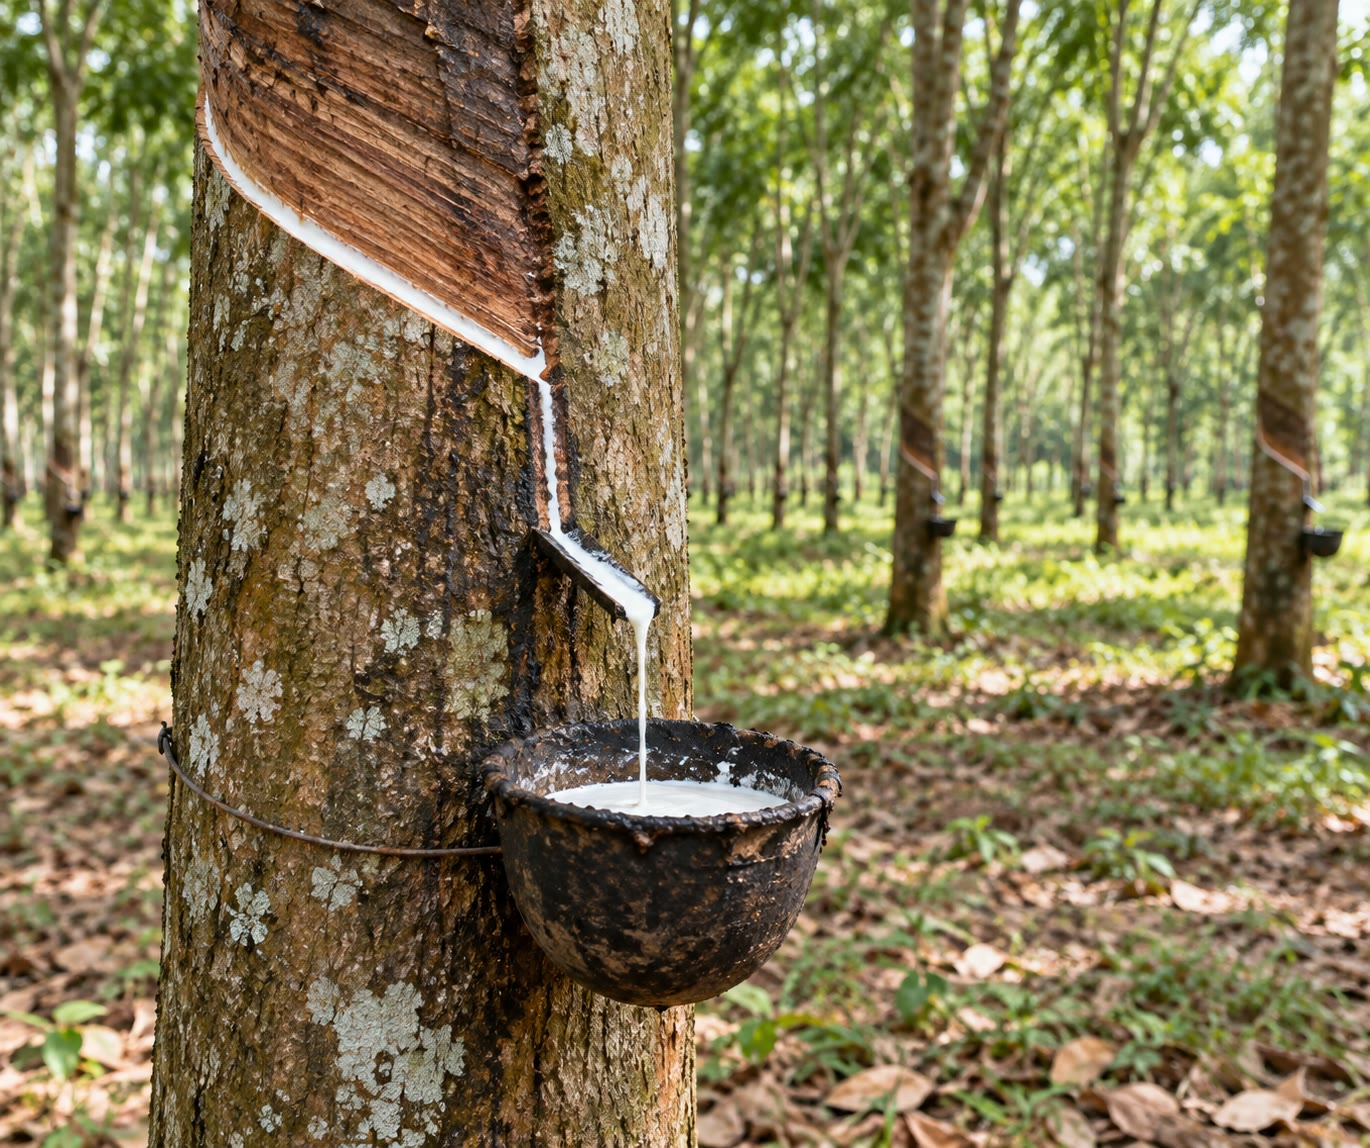
\includegraphics[width=0.45\linewidth]{images/book1/ai/g12-rubber-tapping.jpg}

{\small Menyadap pohon karet: lateks mengalir dari sayatan pada kulit
batang ke dalam sebuah mangkuk.}
\end{omfigure}

\begin{remark}[Membuat dan mengurai]\label{rem:g12:polymers:recycling}
\omterm{def:g8:plastics:thermoplastic}{Termoplastik} dapat dilelehkan dan dibentuk kembali: \omterm{def:g5:raw-materials-and-recycling:recycling}{daur ulang} mekanis.
\omterm{def:g12:polymers:addition-polymer}{Polimer kondensasi} juga dapat diuraikan menjadi \omterm{def:g12:polymers:polymer}{monomer-monomernya}
melalui reaksi kebalikannya, yaitu hidrolisis, dan \omterm{def:g12:polymers:polymer}{monomer-monomer} itu
dibuat menjadi \omterm{def:g12:polymers:polymer}{polimer} baru: \omterm{def:g5:raw-materials-and-recycling:recycling}{daur ulang} kimia. \omterm{def:g8:plastics:thermoplastic}{Termoset} tidak dapat
menjalani keduanya dengan mudah.
\end{remark}

\section{Latihan}

\begin{exercise}[$\star$]\label{exo:g12:polymers:1}
Berikan \omterm{def:g12:polymers:polymer}{monomer} polipropena, yang \omterm{def:g12:polymers:repeat-unit}{unit ulangnya}
\ce{-CH2-CH(CH3)-}.
\end{exercise}

\begin{exercise}[$\star$]\label{exo:g12:polymers:2}
Tuliskan \omterm{def:g12:polymers:repeat-unit}{unit ulang} \omterm{def:g12:polymers:polymer}{polimer} yang dibuat dari tetrafluoroetena,
\ce{CF2=CF2}. Apakah \omterm{def:g12:polymers:polymer}{polimer} itu \omterm{def:g12:polymers:addition-polymer}{polimer adisi} atau \omterm{def:g12:polymers:addition-polymer}{polimer kondensasi}?
\end{exercise}

\begin{exercise}[$\star$]\label{exo:g12:polymers:3}
Golongkan sebagai \omterm{def:g12:polymers:addition-polymer}{polimer adisi} atau \omterm{def:g12:polymers:addition-polymer}{polimer kondensasi}: polietena,
PET, nilon, PVC, polistirena.
\end{exercise}

\begin{exercise}[$\star$]\label{exo:g12:polymers:4}
Manakah di antara \omterm{def:g12:polymers:polymer}{polimer-polimer} ini yang alami: selulosa, nilon, pati,
PVC, karet dari lateks, protein?
\end{exercise}

\begin{exercise}[$\star$]\label{exo:g12:polymers:5}
Mengapa setiap \omterm{def:g12:polymers:polymer}{monomer} sebuah \omterm{def:g12:polymers:addition-polymer}{polimer kondensasi} harus membawa dua gugus
reaktif?
\end{exercise}

\begin{exercise}[$\star\star$]\label{exo:g12:polymers:6}
Sebuah sampel PVC memiliki \omterm{def:g10:the-mole:molar-mass}{massa molar} rata-rata \qty{125000}{g/mol}.
Hitung \omterm{def:g12:polymers:repeat-unit}{derajat polimerisasinya}.
\end{exercise}

\begin{exercise}[$\star\star$]\label{exo:g12:polymers:7}
Sebuah rantai polistirena memiliki \omterm{def:g12:polymers:repeat-unit}{derajat polimerisasi} 2500. Hitung
\omterm{def:g10:the-mole:molar-mass}{massa molarnya}.
\end{exercise}

\begin{exercise}[$\star\star$]\label{exo:g12:polymers:8}
Asam laktat, \ce{CH3-CH(OH)-COOH}, membawa sebuah gugus \omterm{def:g11:functional-groups:alcohol}{alkohol} dan
sebuah gugus asam. Tunjukkan bahwa asam itu dapat membentuk poliester
dengan sendirinya, tuliskan \omterm{def:g12:polymers:repeat-unit}{unit ulangnya}, dan sebutkan \omterm{def:g7:atoms-and-molecules:molecule}{molekul} kecil
yang dilepaskan.
\end{exercise}

\begin{exercise}[$\star\star$]\label{exo:g12:polymers:9}
Jelaskan, dengan gambar susunan rantai, mengapa lembaran kantong lunak
dan bening sedangkan botol susu kaku dan buram.
\end{exercise}

\begin{exercise}[$\star\star$]\label{exo:g12:polymers:10}
Gagang sebuah panci terbuat dari \omterm{def:g8:plastics:thermoplastic}{termoset}, demikian pula kenop tutup
\omterm{def:g8:plastics:plastic}{plastiknya}. Uraikan rantai-rantainya. Mengapa keduanya tidak dapat
dilelehkan dan didaur ulang?
\end{exercise}

\begin{exercise}[$\star\star$]\label{exo:g12:polymers:11}
Sebuah rantai nilon-6,6 memiliki \omterm{def:g10:the-mole:molar-mass}{massa molar} \qty{22600}{g/mol}. Hitung
\omterm{def:g10:the-mole:molar-mass}{massa molar} \omterm{def:g12:polymers:repeat-unit}{unit ulangnya} \ce{C12H22N2O2}, lalu \omterm{def:g12:polymers:repeat-unit}{derajat
polimerisasinya}.
\end{exercise}

\begin{exercise}[$\star\star\star$]\label{exo:g12:polymers:12}
Tuliskan reaksi antara satu \omterm{def:g7:atoms-and-molecules:molecule}{molekul} heksana-1,6-diamina dan satu
\omterm{def:g7:atoms-and-molecules:molecule}{molekul} asam heksanadioat, yang menghasilkan sambungan \omterm{def:g11:functional-groups:amine}{amida} pertama.
Mengapa produknya dapat terus bereaksi di kedua ujungnya?
\end{exercise}

\begin{exercise}[$\star\star\star$]\label{exo:g12:polymers:13}
Berapa massa air yang dilepaskan ketika \qty{1.0}{kg} nilon-6,6
dibuat?
\end{exercise}

\begin{exercise}[$\star\star\star$]\label{exo:g12:polymers:14}
Karet alam lunak dan lengket ketika hangat; jika dipanaskan dengan
belerang, karet itu menjadi karet ban yang elastis dan liat. Jelaskan
dengan rantai-rantainya. Mengapa ban begitu sulit didaur ulang?
\end{exercise}

\begin{exercise}[$\star\star\star$]\label{exo:g12:polymers:15}
Pati dan selulosa memiliki rumus yang sama per satuan, \ce{C6H10O5}.
Sebuah rantai selulosa memiliki \omterm{def:g10:the-mole:molar-mass}{massa molar} \qty{1.6e6}{g/mol}. Berapa
satuan glukosa yang dikandungnya? Berapa panjangnya, jika setiap satuan
menambah \qty{0.5}{nm} pada panjangnya?
\end{exercise}

\section{Soal: Dari Botol menjadi Jaket}

\begin{problem}[{Soal akhir pekan --- berapa botol 25 g yang diperlukan
untuk satu jaket bulu sintetis?}]
\label{pb:g12:polymers:1}
% ledger: aw:C, aw:H, aw:O
Sebuah jaket bulu sintetis dibuat dari \qty{300}{g} serat PET. Botol
bekas yang masing-masing \qty{25}{g} dikumpulkan, dipilah, dicuci,
dicacah, dilelehkan, dan dipintal; dalam proses ini \qty{80}{\percent}
massa botol berakhir sebagai serat di dalam jaket.

\medskip
\noindent\textbf{Bagian I --- \omterm{def:g12:polymers:polymer}{Polimernya}.}
\begin{enumerate}
  \item Sebutkan kedua \omterm{def:g12:polymers:polymer}{monomer} PET dan \omterm{def:g11:functional-groups:functional-group}{gugus fungsi} yang dibawanya.
  \item Sambungan apa yang terbentuk di antara keduanya? \omterm{def:g7:atoms-and-molecules:molecule}{Molekul} kecil
        apa yang dilepaskan?
  \item Apakah PET \omterm{def:g12:polymers:addition-polymer}{polimer adisi} atau \omterm{def:g12:polymers:addition-polymer}{polimer kondensasi}?
  \item Hitung \omterm{def:g10:the-mole:molar-mass}{massa molar} kedua \omterm{def:g12:polymers:polymer}{monomer} itu.
  \item Simpulkan \omterm{def:g10:the-mole:molar-mass}{massa molar} \omterm{def:g12:polymers:repeat-unit}{unit ulang} \ce{C10H8O4}, lalu periksalah
        dengan rumusnya.
\end{enumerate}

\medskip
\noindent\textbf{Bagian II --- Rantai-rantainya.}
\begin{enumerate}[resume]
  \item PET sebuah botol memiliki rantai dengan \omterm{def:g10:the-mole:molar-mass}{massa molar} rata-rata
        \qty{38400}{g/mol}. Hitung \omterm{def:g12:polymers:repeat-unit}{derajat polimerisasinya}.
  \item Kira-kira berapa sambungan \omterm{def:g11:functional-groups:carboxylic-acid}{ester} yang dikandung satu rantai?
  \item PET botol sebagian bersifat kristalin. Apa artinya bagi
        rantai-rantainya?
  \item Mengapa PET dapat dilelehkan dan dipintal menjadi serat?
\end{enumerate}

\medskip
\noindent\textbf{Bagian III --- \omterm{def:g5:raw-materials-and-recycling:recycling}{Daur ulang}.}
\begin{enumerate}[resume]
  \item Berapa massa botol yang diperlukan untuk satu jaket?
  \item Berapa botol itu?
  \item Apa yang terjadi pada sisa massanya?
  \item Prinsip \omterm{def:g12:synthesis-strategy:green-chemistry}{kimia hijau} mana yang diterapkan \omterm{def:g5:raw-materials-and-recycling:recycling}{daur ulang} ini?
\end{enumerate}

\medskip
\noindent\textbf{Bagian IV --- Kembali ke \omterm{def:g12:polymers:polymer}{monomer}.}
\begin{enumerate}[resume]
  \item Tuliskan, untuk satu \omterm{def:g12:polymers:repeat-unit}{unit ulang}, hidrolisis PET menjadi
        \omterm{def:g12:polymers:polymer}{monomer-monomernya}.
  \item Berapa jumlah \omterm{def:g12:polymers:repeat-unit}{unit ulang} dalam \qty{1.00}{kg} PET?
  \item Berapa massa setiap \omterm{def:g12:polymers:polymer}{monomer} yang dihasilkan hidrolisis sempurna
        \qty{1.00}{kg} PET?
  \item Berapa massa air yang dihabiskannya? Periksalah \omterm{def:g8:balanced-equations:conservation}{kekekalan
        massanya}.
  \item Berikan satu keunggulan \omterm{def:g5:raw-materials-and-recycling:recycling}{daur ulang} kimia ini dibandingkan
        pelelehan.
  \item Nyatakan jawaban akhirnya: berapa botol \qty{25}{g} yang
        diperlukan untuk satu jaket bulu sintetis?
\end{enumerate}
\end{problem}
